\documentclass[notes=hide,hyperref={dvipdfmx,pdfpagelabels=false}]{beamer}
\mode<article>
{
  \usepackage{fullpage}
  \usepackage{pgf}
  \usepackage[xetex]{hyperref}
  \setjobnamebeamerversion{beamer}
}

\mode<presentation>
{
  %\usetheme{Frankfurt}
 %\usetheme{My}
  \usetheme{Madrid}
  % or ...
%\usecolortheme{seagull}
  %\setbeamercovered{transparent}
  %\setbeamercovered{dynamic}
  % or whatever (possibly just delete it)
}
\usenavigationsymbolstemplate{}
\usefonttheme{structurebold}
\usepackage{multimedia}
%\usepackage{tikz}
\usepackage{fontspec,xunicode,xltxtra}

%\usepackage{polyglossia}
%\setdefaultlanguage[spelling=new, latesthyphen=true]{german}
%\setsansfont{DejaVu Sans}
%\setsansfont{Verdana}
%\setsansfont{Arial}
%\setromanfont{Linux Libertine O}
%\setsansfont{Linux Biolinum O}

\setbeamertemplate{footline}
{
\leavevmode
%\hbox{\begin{beamercolorbox}[wd=.5\paperwidth,ht=2.5ex,dp=1.125ex,
%leftskip=.3cm plus1fill,rightskip=.3cm]{author in head/foot}%
%    \usebeamerfont{author in head/foot}\insertshortauthor
%  \end{beamercolorbox}%
%  \begin{beamercolorbox}[wd=.5\paperwidth,ht=2.5ex,dp=1.125ex,leftskip=.3cm,
%rightskip=.3cm plus1fil]{title in head/foot}%
%    \usebeamerfont{title in head/foot}\insertshorttitle\hfill

\hfill\insertframenumber  \hspace{3pt}

%\inserttotalframenumber
%\hspace*{2ex}
%  \end{beamercolorbox}}%
  \vskip3pt%
}

\usepackage[ngerman]{babel}
\selectlanguage{ngerman}

%
% math/symbols
%
\usepackage{amssymb}
\usepackage{amsthm}
% \usepackage{latexsym}
\usepackage{amsmath}
%\usepackage{amsxtra} %Weitere Extrasymbole
%\usepackage{empheq} %Gleichungen hervorheben
%\usepackage{bm}
 %\bm{A} Boldface im Mathemodus

\usepackage{cellspace}
\setlength{\cellspacetoplimit}{2pt}
\setlength{\cellspacebottomlimit}{2pt}

%%%%%%%%%%%%%%%%%% Fuer Frames [fragile]-Option verwenden!
%Programm-Listing
%%%%%%%%%%%%%%%%%%
%Listingsumgebung fuer verbatim
%Grauhinterlegeter Text
%Automatischer Zeilenumbruch ist aktiviert
\usepackage{listings}
\definecolor{lgray}{gray}{0.80}
%\lstset{backgroundcolor=\color{lgray}, frame=single, basicstyle=\ttfamily, breaklines=true}
\lstnewenvironment{sage}{\lstset{backgroundcolor=\color{lgray},language=Python, emphstyle=\color{red}, frame=single, basicstyle=\ttfamily, breaklines=true,mathescape =true,escapechar=§}}{}


\usepackage{mydef}
%\usepackage{cmap} % you can search in the pdf for umlauts and ligatures
\usepackage{colonequals} %corrects the definition-symbols \colonequals (besides others)
\title{Einführung in Sage}
%
%\subtitle{Disputation} % (optional)

\author{Jochen Schulz}
% - Use the \inst{?} command only if the authors have different
%   affiliation.

\institute{Georg-August Universit\"at G\"ottingen \pgfimage[height=0.5cm]{../figures/unilogo3}}
% - Use the \inst command only if there are several affiliations.
% - Keep it simple, no one is interested in your street address.

\date{\today}

\subject{Sage}
% This is only inserted into the PDF information catalog. Can be left
% out. 

% If you have a file called "university-logo-filename.xxx", where xxx
% is a graphic format that can be processed by latex or pdflatex,
% resp., then you can add a logo as follows:

%\logo{\pgfimage[height=0.5cm]{figures/unilogo3}}


% Delete this, if you do not want the table of contents to pop up at
% the beginning of each subsection:

\AtBeginSection[]
{
  \begin{frame}<beamer>
    \frametitle{Aufbau}
    \tableofcontents[currentsection,currentsubsection]
  \end{frame}
}

\AtBeginSubsection[]
{
  \begin{frame}<beamer>
    \frametitle{Aufbau}
    \tableofcontents[currentsection,currentsubsection]
  \end{frame}
}



%%%%%%%%%%%%%%%%%%%
%Neue Definitionen
%%%%%%%%%%%%%%%%%%%

%Newcommands
\newcommand{\Fun}[1]{\mathcal{#1}}      %Mathcal fuer Funktoren
\newcommand{\field}[1]{\mathbb{#1}}     %Grundkoerper ?? in mathds

\newcommand{\A}{\field{A}}              %Affines A
\newcommand{\C}{\field{C}}              %Complexes C
\newcommand{\Fp}{\field{F}_{\!p}}       %Endlicher Koerper mit p Elementen
\newcommand{\Fq}{\field{F}_{\!q}}       %Endlicher Koerper mit q Elementen
\newcommand{\Ga}{\field{G}_{a}}         %Add Gruppenschema
\newcommand{\K}{\field{K}}              %Generischer Koerper 
\newcommand{\N}{\field{N}}              %Nat Zahlen
\newcommand{\Pj}{\field{P}}             %Projektives P
\newcommand{\R}{\field{R}} 		%Reelle Zahlen
\newcommand{\Q}{\field{Q}}              %Rationale Zahlen  
\newcommand{\Qt}{\field{H}}             %Quaternionen 
\newcommand{\V}{\field{V}}              %Vektorbuendel V
\newcommand{\Z}{\field{Z}}              %Ganze Zahlen

\newcommand{\fdg}{\;|\;}                 %fuer die gilt

%Operatoren
\DeclareMathOperator{\Abb}{Abb}
%\usepackage{sagetex}

\begin{document}
\lstset{basicstyle={\lstbasicfont\footnotesize}}


\subtitle{Einheit 6}
\maketitle

\begin{frame}{Aufbau}
\tableofcontents
\end{frame}

% \begin{frame}[fragile]{Übersicht}
% \begin{itemize}
% \item Nachtrag
% \item Folgen, Konvergenz von Folgen
% \item Realisierung in MuPAD
% \item Reihen, Konvergenzkriterien
% \item Potenzreihen
% \item Exponentialfunktion, Logarithmus, Sinus, Cosinus, Tangens
% \item Schleifen I
% \end{itemize}
% \end{frame}

\begin{frame}[fragile]{Datentypen}
\begin{enumerate}
\item Bezeichner -- \verb+DOM_IDENT+
\item Ausdrücke -- \verb+DOM_EXPR+
\item Ganze Zahlen -- \verb+DOM_INT+
\item Rationale Zahlen -- \verb+DOM_RAT+
\item Complexe Zahlen -- \verb+DOM_COMPLEX+
\item Gleitkommazahlen -- \verb+DOM_FLOAT+
\item Mengen -- \verb+DOM_SET+
\item Listen -- \verb+DOM_LIST+
\item Matrizen -- \verb+Dom::Matrix()+
\item Tabellen -- \verb+DOM_TABLE+
\item Arrays -- \verb+DOM_ARRAY+
\item Funktionen/Prozeduren -- \verb+DOM_PROC+
\item Zeichenketten -- \verb+DOM_STRING+
\end{enumerate}
\end{frame}

%===================================================
\section{Folgen}
%==================================================

\begin{frame}{Folgen}
\begin{itemize}
\item Eine {\color{red} reelle Zahlenfolge} kurz {\color{red} Folge} genannt, ist eine
Abbildung von $\mathbb{N}$ in $\mathbb{R}$.
\item Statt $a:\mathbb{N} \ \rightarrow \ \mathbb{R}$ schreibt man in
Anlehnung an die Vektornotation $(a_n)_{n \in \mathbb{N}}$ oder einfach $(a_n)_{n}$.
\item Natürlich kann man auch Folgen $\mathbb{N} \ \rightarrow \ Y$ auf beliebigen Mengen $Y$
betrachten. Aber wir beschränken uns auf den Fall $Y=\mathbb{R}$. 
\item Die Zahlen $a_n$ heißen {\color{red} Glieder} der Folge.
\item Eine {\color{red} Teilfolge} $(a_{n_i})_{n_i}$ ist eine Abbildung $a:N \
\rightarrow \ \mathbb{R}$, wobei $N \subset \mathbb{N}$ eine Menge mit
unendlich vielen Elementen ist.
\end{itemize}
\end{frame}

\begin{frame}{Konvergenz von Folgen}
Eine Zahlenfolge $(a_n)_n$ ist {\color{red} konvergent} gegen den {\color{red}
Grenzwert} oder {\color{red} Limes} $a\in \mathbb{R}$, wenn es zu jedem
$\varepsilon >0$ ein $n_0 \in \mathbb{N}$ gibt, so dass für alle $n \geq
n_0$ die Abschätzung 
\[ |a_n - a|< \varepsilon \]
 gilt. Man schreibt
\[ a=\lim_{n \rightarrow \infty} a_n. \]
Eine nicht konvergente Folge nennt man {\color{red} divergent}. 
\end{frame}


\begin{frame}{Bemerkungen}
\begin{itemize}
\item Konvergiert eine Folge gegen $0$, so nennt man sie eine
\alert{Nullfolge}.
\item Der Grenzwert einer konvergenten Teilfolge $(a_{n_i})_{n_i}$
 heißt {\color{red} Häufungspunkt}. 
\item Ein Folge kann keinen aber auch mehrere Häufungspunkte besitzten; konvergente Folgen haben genau einen Häufungspunkt.
\item  Eine {\color{red} Cauchy-Folge} ist eine Folge $(a_n)_n$ bei der für
alle $\varepsilon>0$ ein $n_0 \in \mathbb{N}$ existiert, so dass für alle
$n,m \geq n_0$ gilt:
$|a_n - a_m| < \varepsilon$. \\
In $\mathbb{R}$ ist eine Folge konvergent,
genau dann wenn sie eine Cauchy-Folge ist (Vollständigkeit).
\item Eine {\color{red} $\varepsilon$-Umgebung} $U_\varepsilon(a)$ von $a$ ist
definiert durch
\[
U_\varepsilon(a) := (a-\varepsilon, a+\varepsilon) := \{ x \in \mathbb{R} \ | \ |x - a| < \varepsilon \}.
\] 
\end{itemize}
\end{frame}

\begin{frame}{Beispiele}
\begin{tabular}{SlSlSl}
$a_n:= \frac{1}{n+1}$ & $1, \frac{1}{2}, \frac{1}{3}, \frac{1}{4}, \ldots$\\
$b_n:= 2^{-n}$ & $1,\frac{1}{2}, \frac{1}{4}, \frac{1}{8}, \ldots$\\
$c_n:=2^n$ & $1,2,4,8,\ldots$\\
$d_n:=\left( \frac{n+2}{n+1} \right)^{n+1}$ & $\frac{2^1}{1^1},
\frac{3^2}{2^2}, \frac{4^3}{3^3},...$\\
$e_n=(-1)^n$ & $1,-1,1,-1,...$\\
\end{tabular}
\bigskip

Die Folgen
$(a_n)_n$, $(b_n)_n$ und  $(d_n)_n$ konvergieren und $(c_n)_n$,
$(e_n)_n$ divergieren. 
\end{frame}

\begin{frame}[fragile]{Folgen in Sage I}
Grenzwerte von Folgen $(a_n)_n$ können in Sage mit Hilfe von 
\begin{sage}
>> limit(expr(x), x = oo, dir='above')
\end{sage}
berechnet werden. Dabei ist $expr(x)$ ein Ausdruck.

\textbf{Beispiele:}
\begin{sage}
>> _=var('n');limit(1/(n+1),n=oo)
\end{sage}
\begin{sage}
  0
\end{sage}
\begin{sage}
>> limit(((n+2)/(n+1))^(n+1),n=oo)
\end{sage}
\begin{sage}
  e
\end{sage}
\begin{sage}
>> limit((-1)^n,n=oo)
\end{sage}
\begin{sage}
  ind
\end{sage}
\end{frame}

\begin{frame}[fragile]{Folgen in Sage II}
\begin{sage}
>> limit(2^n,n=oo)
\end{sage}
\begin{sage}
  +Infinity
\end{sage}
\begin{sage}
>> lim(x*sin(1/x), x=0)
\end{sage}
\begin{sage}
  0
\end{sage}
\end{frame}

\begin{frame}[fragile]{Visualiseren von Folgen}
Folgen können in Sage durch {\color{blue} \verb+points+} visualisiert werden.
\begin{sage}
>> var('n');
>> point([(n,(-1)^n/n) for n in range(1,21)], pointsize=8)
\end{sage}
\begin{center}
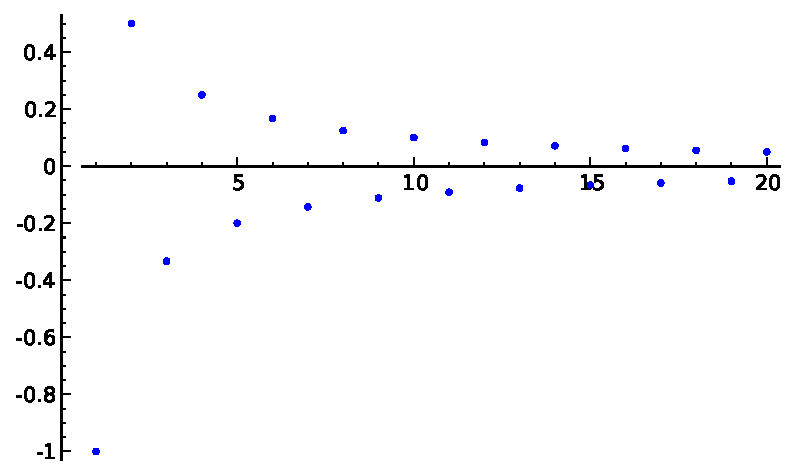
\includegraphics[width=9.5cm]{figures/folge.pdf}
\end{center}
\end{frame}

\begin{frame}{Konvergenzkriterien}
\begin{itemize}
\item Jede monotone, beschränkte Folge konvergiert.
\item Sind $(a_n)_n$ und $(b_n)_n$ konvergente Folgen, $\alpha, \beta \in \mathbb{R}$, so ist auch die
                   Folge $( \alpha a_n+\beta b_n)_n$ konvergent mit
                   dem Grenzwert
 \[ \lim_{n \rightarrow \infty} ( \alpha a_n + \beta b_n)= \alpha
                   \lim_{n \rightarrow \infty} a_n + \beta \lim_{n
                   \rightarrow \infty} b_n .\]
\item Sind $(a_n)_n$ und $(b_n)_n$ konvergente Folgen, so ist auch die
                   Folge $(a_n b_n)_n$ konvergent mit
                   dem Grenzwert
 \[
  \lim_{n \rightarrow \infty} ( a_n b_n)= 
                   (\lim_{n \rightarrow \infty} a_n) \cdot  (\lim_{n
                   \rightarrow \infty} b_n).
 \]
\item Weglassen oder Hinzufügen endlich vieler Glieder verändert das
                   Konvergenzverhalten nicht.
\end{itemize}
\end{frame}

\begin{frame}{Wichtige Sätze}
\begin{itemize}
\item (Bolzano-Weierstrass) Jede beschränkte Folge besitzt (mindestens) eine
konvergente Teilfolge.
\item Jede Teilfolge einer konvergenten Folge konvergiert gegen den
Grenzwert der ursprünglichen Folge.
\item Jede konvergente Folge ist beschränkt, d.h. es gibt ein $K>0$,
so dass $|a_n|\leq K$ gilt für alle $n \in \mathbb{N}$.
\item Seien $(a_n)_n$ und $(b_n)_n$ konvergente Folgen mit $\lim_{n
\rightarrow \infty} a_n = \lim_{n \rightarrow \infty} b_n$. Dann gilt
für eine Folge $(c_n)_n$ mit $a_n \leq c_n \leq b_n$, $n \in
\mathbb{N}$, dass sie konvergiert mit  $\lim_{n
\rightarrow \infty} c_n = \lim_{n \rightarrow \infty} b_n$.
\end{itemize}
\end{frame}

\begin{frame}[fragile]{Rekursive Folgen}
Rekursive Folgen können durch rekursive Funktionen erzeugt werden.
\textbf{Beispiel:}
\[ y_{n+2}:=2y_{n+1}-y_n+2, \quad y_0=-1, y_1=a. \]
\begin{sage}
>>var('a')
>>def y(n):
>>    if n==0:
>>        return -1
>>    if n==1:
>>        return a
>>    return 2*y(n-1)-y(n-2)+2
\end{sage}
\begin{sage}
4*a + 15
\end{sage}
\end{frame}

%===============================================
\section{Reihen}
%===============================================

\begin{frame}{Reihen}
Sei $(a_n)_n$ eine Folge reeller Zahlen. Eine {\color{red} (unendliche)
Reihe} mit den {\color{red} Gliedern} $a_n$, in Zeichen
\[ \sum_{n=1}^\infty a_n =a_1 + a_2 + a_3 + \dots, \]
ist definiert durch die Folge $(s_n)_n$ der {\color{red} Partialsummen}\\
\centering{$s_n=\sum_{k=1}^n a_k = a_1+a_2+ \dots +a_n$.}\\
Der Grenzwert $s$ der Folge $(s_n)_n$ wird als {\color{red} Wert} oder {\color{red}
Summe} der Reihe bezeichnet. Man schreibt
\[s= \sum_{n=1}^\infty a_n.\] 
\end{frame}

\begin{frame}{Bemerkungen}
\begin{itemize}
\item Beginnt die Indizierung statt bei $1$ mit einer anderen ganzen
Zahl $m$, so wird $\sum_{n=m}^\infty a_n$ entsprechend eingeführt.
\item Bei Abänderung, Weglassen oder Hinzufügen endlich vieler Glieder
bleiben Konvergenz und Divergenz unberührt. I.A. wird sich aber der
Grenzwert ändern.
\item  Reihen sind eine spezielle Art von Folgen.
\end{itemize}
\end{frame}

\begin{frame}{Beispiele I}
\begin{itemize}
\item Die \alert{geometrische Reihe} ist gegeben durch $\sum_{n=0}^\infty x^n$. Die
Partialsummen lauten
\[ s_n=1+x+x^2+\ldots + x^n = \left \{ \begin{array}{ll}
n+1, & \mbox{ falls } x=1\\
\frac{1-x^{n+1}}{1-x}, & \mbox{ falls } x \neq 1 
\end{array} \right. .\]
Also divergiert die Reihe für $|x|\geq1$ und konvergiert für $|x|<1$ mit
dem Wert $\sum_{n=0}^\infty = \frac{1}{1-x}$.

\item Die Reihe $\sum_{n=1}^\infty \frac{1}{n^2}$ konvergiert gegen
$\pi^2/6$.
 \end{itemize}
\end{frame}

\begin{frame}{Beispiele II}
\begin{itemize}
\item Die \alert{harmonische Reihe} $\sum_{n=1}^\infty \frac{1}{n}$
 divergiert.
\item Die \alert{alternierende harmonische Reihe}  $\sum_{n=1}^\infty
\frac{(-1)^{n+1}}{n}$ konvergiert.
\item Die Reihe  $\sum_{n=1}^\infty \frac{1}{n^s}$ konvergiert für $s>1$.
\item Die Reihe  $\sum_{n=2}^\infty \frac{1}{n(\log n)^s}$ konvergiert
für $s>1$ und divergiert für $s=1$.
\end{itemize}
\end{frame}

\begin{frame}[fragile]{Reihen mit Sage I}
Der Befehl {\color{blue} \verb+sum(f,i=a..b)+} sucht eine geschlossene
Darstellung der Summe $\sum_{i=a}^b f(i)$. Dabei sind $a$,$b$ ganze
 Zahlen, wobei auch unendlich (also \verb+infinity+) erlaubt
ist und \verb+f+ ist ein Ausdruck in $i$.
\begin{sage}
>> _=var('k');sum(1/k^2,k,1,oo)
\end{sage}
\begin{small}
\begin{sage}
1/6*pi^2
\end{sage}
\end{small}
\begin{sage}
>> sum((-1)^(k+1)/k,k,1,oo)
\end{sage}
\begin{sage}
  log(2)
\end{sage}
\begin{sage}
>> sum(1/k,k,1,oo)
\end{sage}
\begin{sage}
ValueError: Sum is divergent
\end{sage}
\end{frame}


\begin{frame}[fragile]{Reihen mit Sage II}
Oft ist die Konvergenz einer Reihe abhängig von bestimmten Parametern,
wie z.B. bei der geometrischen Reihe. Und je nach Parameterwert zeigt die Reihe
unterschiedliches Konvergenzverhalten
\begin{sage}
>> sum(x^k,k,0,oo)
\end{sage}
\begin{sage}
Is  abs(x)-1  positive, negative, or zero?
\end{sage}
Entsprechend gibt es keine geschlossene Form. Für $x=1/2$ gilt jedoch
\begin{sage}
>> x = 1/2; sum(x^k,k,0,oo)
\end{sage}
\begin{sage}
  2
\end{sage}
\end{frame}

\begin{frame}[fragile]{Etwas mehr Sage}
\begin{itemize}
\item Definieren der Partialsumme
\begin{sage}
>> del x;_=var('x,n')
>> s = sum(x^k,k,0,n); s
\end{sage}
\begin{small}
\begin{sage}
(x^(n + 1) - 1)/(x - 1)
\end{sage}
\end{small}
\item Die ersten $5$ Glieder der Partialsumme
\begin{sage}
>> assume(x<>1); [s(n=m) for m in [1..6]]
\end{sage}
\begin{sage}
[(x^2 - 1)/(x - 1), (x^3 - 1)/(x - 1), (x^4 - 1)/(x - 1), (x^5 - 1)/(x -
1), (x^6 - 1)/(x - 1), (x^7 - 1)/(x - 1)]
\end{sage} 
 \end{itemize}
\end{frame}

\begin{frame}[fragile]{Etwas mehr Sage II}
\begin{itemize}
\item Bestimmen des Grenzwertes der Folge der Partialsummen
\begin{sage}
>> forget();assume(abs(x)<1);limit(s,n=oo)
\end{sage}
\begin{sage}
-1/(x - 1)
\end{sage}
\begin{sage}
>> forget();assume(x>1);limit(s,n=oo)
\end{sage}
\begin{sage}
+Infinity
\end{sage}
\end{itemize}
\end{frame}

\begin{frame}[fragile]{assume}
Mit der Funktion \verb+assume+ kann man Funktionen wie \verb+expand+,
\verb+simplify+ oder  \verb+solve+ mitteilen, dass für gewisse Bezeichner
Annahmen über ihre Bedeutung gemacht wurden. 

\textbf{Beispiele:}
 
{\color{blue} 
\begin{tabular}{ll}
\verb+assume(x,'real')+ & $x$ wird auf $\mathbb{R}$ eingeschränkt!\\
\verb+assume(x>a)+ & $x$ wird auf  $\{y \in \mathbb{R}\ |\ y>a\}$
eingeschr"ankt!
\end{tabular}
}

Ruft man \verb+assume+ mehrmals für einen Bezeichner auf, werden zusätzliche Annahmen gemacht. Sind diese
Widersprüchlich erhält man eine entsprechende Meldung.
\end{frame}

\begin{frame}[fragile]{Bemerkungen}
\begin{itemize}
\item Umformungen oder Vereinfachungen für symbolische Bezeichner
werden i.A. nur dann durchgeführt,
wenn sie für alle komplexen Zahlen gelten. Hier kann ein Einschränken
des Definitionsbereichs helfen.
\item Mittels {\color{blue} \verb+forget(x>a)+} wird die Annahme \verb+x>a+ gelöscht.
\item Durch {\color{blue} \verb+assumptions()+} können alle Annahmen ausgegeben werden.
%\item Durch den speziellen Bezeichner \verb+Global+ können Annahmen
%für alle Bezeichner gesteuert werden. 
\end{itemize}
\end{frame}

\begin{frame}[fragile]{Beispiele zu assume I}
\begin{sage}
>> var('c'); assumptions()
\end{sage}
\begin{sage}
c
[]
\end{sage}

\begin{sage}
>> c = 2; assume(c>0)
\end{sage}
\begin{sage}
 AttributeError: 'bool' object has no attribute 'assume'
\end{sage}
\end{frame}

\begin{frame}[fragile]{Beispiele zu assume II}
\begin{sage}
>> del c;_=var('c')
>> assume(c,'integer'); assumptions()
\end{sage}
\begin{sage}
[c is integer]
\end{sage}
\begin{sage}
>> sin(c*pi)
\end{sage}
\begin{sage}
sin(pi*c)
\end{sage}
\begin{sage}
>> sin(c*pi).simplify()
\end{sage}
\begin{sage}
   0
\end{sage}
\end{frame}

\begin{frame}[fragile]{Beispiele zu assume III}

\begin{sage}
>> assume(x>0)
>> sqrt(x^2).simplify()
\end{sage}
\begin{sage}
  x
\end{sage}
\begin{sage}
>> ??
\end{sage}
\begin{sage}
  
\end{sage}
\begin{sage}
>> ??
\end{sage}
\begin{sage}
  
\end{sage}
\begin{sage}
>>
\end{sage}
\begin{sage}

\end{sage}
\end{frame}

\begin{frame}[fragile]{Einige Grundbereiche ??}
\begin{tabular}{|l|l|}
\hline
Grundbereich & Erklärung\\
\hline
\verb+Type::Real+ & $\mathbb{R}$ \\
\verb+Type::Rational+ & $\mathbb{Q}$\\
\verb+Type::Integer+ &  $\mathbb{Z}$\\
\verb+Type::Prime+   & Primzahlen \\
\verb+Type::+ \verb+Intervall(a,b,T)+ & $\{ x \in T | a < x < b\}$, 
$T$ Grundbereich \\
\verb+Type::Positive+ & $\mathbb{R}_+$ \\
\verb+Type::NonZero+ & $\mathbb{C} \smallsetminus \{ 0 \}$\\
\verb+Type::NegRat+ & $\mathbb{Q}_-$\\
\hline
\end{tabular}
\end{frame}

\begin{frame}{Konvergenzkriterien}
\begin{itemize}
\item \alert{Cauchykriterium:} Eine Reihe $\sum_{n=1}^\infty a_n$ konvergiert
                  genau dann, wenn es zu jedem $\varepsilon>0$ ein $n_0
                  \in \mathbb{N}$ gibt, so dass für alle $m,n \geq n_0$
                  gilt $| \sum_{k=m}^n a_k|<\varepsilon$.
\item \alert{Notwendiges Kriterium:} Konvergiert eine Reihe, so bilden ihre Glieder eine Nullfolge. Dieses Kriterium ist \alert{nicht} hinreichend!
\item \alert{Verdichtungskriterium:} Eine Reihe $\sum_{n=1}^\infty a_n$ mit
                  einer Folge nichtnegativer, monoton fallender
                  Glieder konvergiert genau dann, wenn die Reihe
                  $\sum_{n=1}^\infty 2^n a_{2^n}$ konvergiert.
\end{itemize}
\end{frame}

\begin{frame}{Majorantenkriterium}
\begin{itemize}
\item Gilt $0 \leq c_n \leq a_n \leq b_n$ für alle $n \in \mathbb{N}$,
                  so nennt man  $\sum_{n=1}^\infty c_n$ eine {\color{red}
                  Minorante} und   $\sum_{n=1}^\infty b_n$ eine {\color{red}
                  Majorante} von $\sum_{n=1}^\infty a_n$.
\item Besitzt eine Reihe mit nichtnegativen Gliedern eine konvergente
                  Majorante, so konvergiert sie.
\item Besitzt  eine Reihe mit nichtnegativen Gliedern dagegen eine divergente Minorante, so divergiert
sie.
\end{itemize}
\end{frame}

\begin{frame}{Konvergenzkriterien}
Die Reihe $\sum_{n=1}^\infty a_n$ konvergiert, wenn...
\begin{description}
\item[Quotientenkriterium:] Die Glieder positiv sind und ein $q<1$
existiert, so dass für $n \in \mathbb{N}$ gilt $\frac{a_{n+1}}{a_n}
\leq q$. 
\item[Wurzelkriterium:] Die Glieder positiv sind und ein $q<1$
existiert, so dass für $n \in \mathbb{N}$ gilt $\sqrt[n]{a_n} \leq
q$. 
\item[Leibnizsches Kriterium:] Die Reihe $\sum_{n=1}^\infty (-1)^n a_n$
konvergiert, wenn die Folge $(a_n)_n$ eine monoton
fallende  Nullfolge ist.
\end{description}
\end{frame}

\begin{frame}[fragile]{Beispiele}
\begin{itemize}
\item Betrachte $\sum_{n=0}^\infty n^4 e^{-n^2}$
\begin{sage}
>> f(n) = n^4.*exp(-n*n)
>> g(n) = f(n+1)/f(n)
>> limit(g(n),n=oo)
\end{sage}
\begin{sage}
  0
\end{sage}
\item Betrache $\sum_{n=2}^\infty \frac{1}{n (\log n)^2}$
\begin{sage}
>> f(n) = 1/(n*(ln(n)^2))
>> g(n) = 2^n*f(2^n)
>> h(n) = 2^n*g(2^n)
>> limit(h(n+1)/h(n),n=oo)
\end{sage}
\begin{sage}
  1/2
 \end{sage}
\end{itemize}
\end{frame}

\begin{frame}{Absolute und bedingte Konvergenz}
Eine Reihe $\sum_{n=0}^\infty a_n$ heißt {\color{red} absolut konvergent}
genau dann wenn $\sum_{n=0}^\infty |a_n|$ konvergiert. 

Eine
konvergente, aber nicht absolut konvergente Reihe heißt {\color{red} bedingt
konvergent}.
\begin{itemize}
\item Absolut konvergente Reihen können beliebig umgeordnet werden.
\item Dies ist i.d.R. bei nicht absolut konvergenten Reihen falsch!
\end{itemize}
\end{frame}

%===============================================
\section{Potenzreihen}
%===============================================


\begin{frame}{Potenzreihen}
Eine {\color{red} Potenzreihe} ist eine Reihe  der Form
\[ \sum_{n=0}^\infty a_n (x-x_0)^n \]
mit $x_0 \in \mathbb{R}$. Das Konvergenzverhalten für verschiedene $x$ wird durch den
{\color{red} Konvergenzradius} 
\[  \rho := \frac{1}{ \limsup _{n \rightarrow \infty} \sqrt[n]{|a_n|}}
\]
bestimmt. Für $|x -x_0|< \rho$ konvergiert die Potenzreihe absolut und für
$|x-x_0|>\rho$ divergiert sie. 
\end{frame}

\begin{frame}{Bemerkungen}
\begin{itemize}
\item Ist $a_n \neq 0$ für alle $n > n_0$, dann gilt für den Konvergenzradius:
\[
 \rho = \limsup _{n \rightarrow \infty} \frac{|a_{n}|}{|a_{n+1}|}.
\]

\item 
Potenzreihen
konvergieren innerhalb ihres Konvergenzradius absolut.
\item Die Konvergenz an den Stellen $x_0-\rho$ und $x_0+\rho$ muss bei
jeder Reihe individuell geprüft werden.   
\item Potenzreihen sind ein mächtiges Werkzeug innerhalb der
Mathematik. 
\end{itemize}
\end{frame}

\begin{frame}[fragile]{Beispiele}
\begin{itemize}
\item $\sum_{n=1}^\infty \frac{x^n}{n!}$
\begin{sage}
>> f(n) = 1/factorial(n)
>> rho = limit(expand(f(n+1)/f(n)),n=oo); rho
\end{sage}
\begin{sage}
  0
\end{sage}
Die Potenzreihe konvergiert für alle $x \in \mathbb{R}$. 
\item $\sum_{n=0}^\infty n^s x^n$, $s>0$
\begin{sage}
>> _=var('s');f(n)= n^s; assume(s>0)
>> limit(expand(f(n)^(1/n)),n=infinity)
\end{sage}
\begin{sage}
  1
\end{sage}
Der Konvergenzradius ist $1$.
\end{itemize}
\end{frame}   

\begin{frame}[fragile]{Exponentialfunktion}
Wir erklären die \alert{Exponentialfunktion} durch
\[  exp(x) := \sum_{i=0}^\infty \frac{x^n}{n!}= 1 + \frac{x}{1!} +
\frac{x^2}{2!}+ \frac{x^3}{3!}+ \dots, x \in \mathbb{R}. \]
 Die Funktion ist auf ganz $\mathbb{R}$ definiert. Plot:
\begin{sage}
>> plot(exp,(-5,5))
\end{sage}
\begin{center}
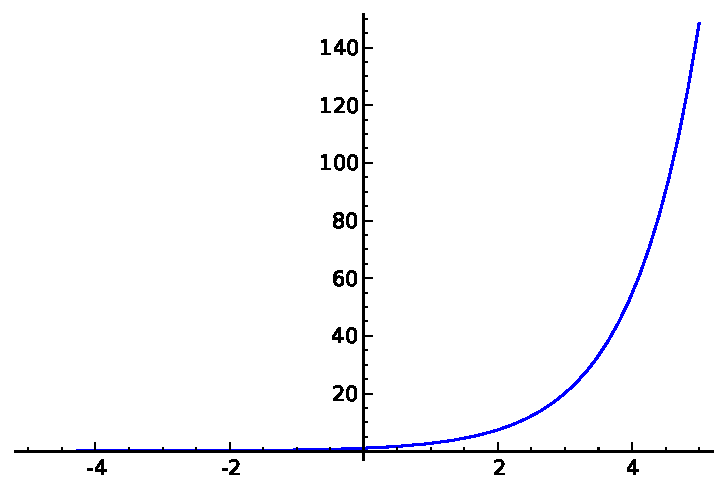
\includegraphics[width=6cm]{figures/fexp.pdf}
\end{center}
\end{frame}

\begin{frame}{Eigenschaften der Exponentialfunktion}
\begin{itemize}
\item Es gilt $\exp(x+y)=\exp(x) \cdot \exp(y)$.
\item Es gilt $\exp(x)=\lim_{n \rightarrow \infty} (1+\frac{x}{n})^n$.
\item Es gilt $\exp(x)=1/\exp(-x)$.
\item Die Umkehrfunktion auf $\mathbb{R}_+$ der Exponentialfunktion ist die
Logarithmusfunktion $\log (x)$. Es gilt
\[ \exp(\log(x))=x, \ x >0, \quad \log ( \exp ( x ))=x, \ x \in \mathbb{R}.\] 
\item Die {\color{red} allgemeine Potenz} ist durch $a^x:=\exp( x \log a)$,
$a\in \mathbb{R}_+$
definiert. 
\end{itemize}
\end{frame}

\begin{frame}[fragile]{Sage}
\begin{sage}
>> sum(x^n/factorial(n),n,0,oo)
\end{sage}
\begin{sage}
  e^x
\end{sage}
\begin{sage}
>> exp(log(x))
\end{sage}
\begin{sage}
  x
\end{sage}
\begin{sage}
>>  ??
\end{sage}
\begin{sage}
  
\end{sage}
\begin{sage}
>> ??
>> ??
\end{sage}
\begin{sage}
  
\end{sage}
\end{frame}

\begin{frame}[fragile]{Trigonometrische Funktionen}
Die {\color{red} Sinusfunktion} und die {\color{red} Cosinusfunktion} sind definiert
durch
\begin{eqnarray*}
\sin(x) := \sum_{n=0}^\infty (-1)^n \frac{x^{2n+1}}{(2n+1)!} \quad\quad
\cos(x) := \sum_{n=0}^\infty (-1)^n \frac{x^{2n}}{(2n)!}. 
\end{eqnarray*}
Die Potenzreihen konvergieren für alle $x \in \mathbb{R}$. Plotten:
\begin{sage}
p = plot(sin,0,4*pi,color='red')
p += plot(cos,0,4*pi); 
p += text('-- $\sin(x)$', (10, 1.0), color='red')
p += text('-- $\cos(x)$', (10, 0.85)); p.show()
\end{sage}
\begin{center}
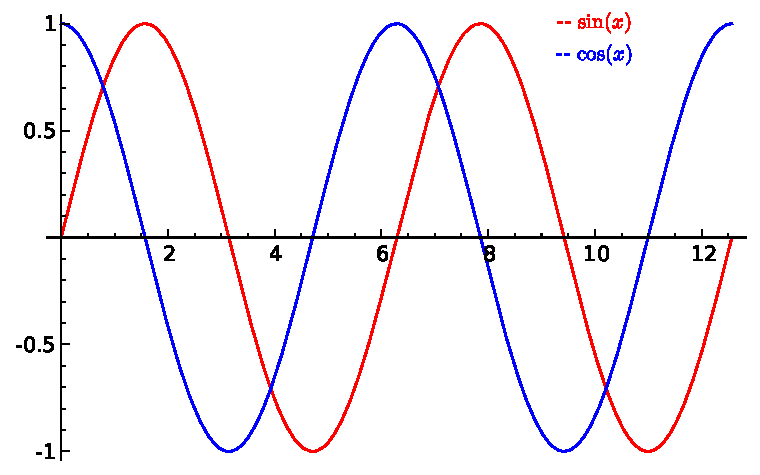
\includegraphics[width=5.5cm]{figures/sincos.pdf}
\end{center}
\end{frame}

\begin{frame}{Eigenschaften}
\begin{itemize}
\item Es gelten die Additionstheoreme:
\begin{eqnarray*}
\sin(x+y) & = &\sin x \cos y+ \cos x \sin y \\
\cos(x+y) & = &\cos x \cos y - \sin x \sin y .
\end{eqnarray*} 
\item Es gilt: 
\[\sin^2x +\cos^2x=1.\]
\item Wir definieren $\pi$, indem wir die kleinste positive Nullstelle
von $\cos(x)$ als $\pi/2$ definieren.
\item Es gilt: 
\begin{eqnarray*}
\sin(x+\pi/2)&=&\cos(x)\\
 \cos(x+\pi/2)&=&-\sin(x).
\end{eqnarray*} 
\end{itemize}
\end{frame}

\begin{frame}[fragile]{Sage}
\begin{sage}
>> solve(cos(x)==0,x)
\end{sage}
\begin{sage}
[x == 1/2*pi]
\end{sage}
\begin{sage}
??
\end{sage}
\begin{sage}
??
\end{sage}
\end{frame}

\begin{frame}[fragile]{Weitere Eigenschaften I}
\begin{itemize}
%\item Man kann die Sinusfunktion und die Cosinusfunktion mit Hilfe eines rechtwinkligen Dreiecks im Einheitskreis auch geometrisch  deuten.
\item Die Umkehrfunktionen von Sinus und Cosinus werden mit $\arcsin$
und $\arccos$ bezeichnet. In Sage: \verb+arcsin+ und \verb+arccos+. 
Plotten: 
\begin{sage}
>> p = plot(arcsin,-1,1,color='red')
>> p += plot(arccos,-1,1); 
>> p += text('-- $arcsin(x)$', (-0.7, 1.0), color='red')
>> p += text('-- $arccos(x)$', (-0.7, 0.75)); p.show()
\end{sage}
\begin{center}
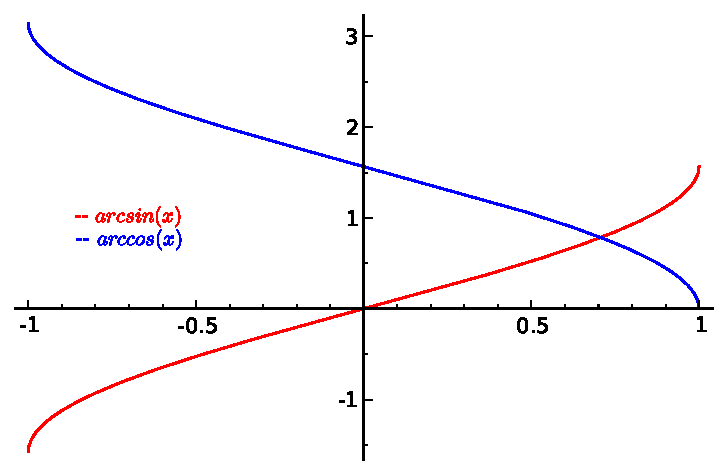
\includegraphics[width=5.5cm]{figures/arcsinarccos.pdf}
\end{center}
\end{itemize}
\end{frame}

\begin{frame}[fragile]{Weitere Eigenschaften II}
\begin{itemize}
\item Der {\color{red} Tangens} ist definiert durch
$\tan(x) :=\frac{\sin(x)}{\cos(x)}$.
\begin{sage}
>> plot(tan,-4,4,detect_poles=True,ymax=4,ymin=-4)
\end{sage}
\begin{center}
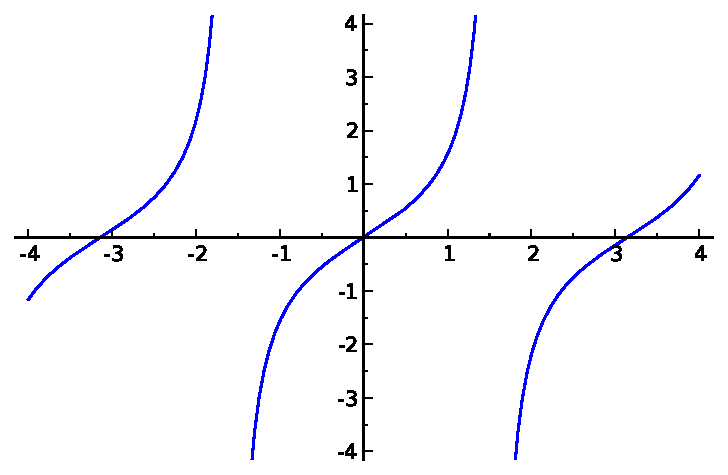
\includegraphics[width=7cm]{figures/tan.pdf}
\end{center}
\end{itemize}
\end{frame}

%-----------
\section{Schleifen I- sollte schon in einheit 2 besprochen werden ?}
%-------------------

\begin{frame}[fragile]{Schleifen I}
Wir kennen bereits Schleifen durch das \verb+[.. for ..]+-Konstrukt. Mit \verb+for+ können aber auch
ganze Blöcke wiederholt werden.
\begin{sage} 
for k in [1..4]:
    x = k^2
    print("Das Quadrat von {0} ist {1}").format(k,x)
\end{sage}
\end{frame}

\begin{frame}[fragile]{Schleifen II}
\begin{itemize}
\item Die Schleifenvariable $k$ durchläuft die Werte $1$, $2$, $3$ und
  $4$. Dabei wird alles was ab \verb+:+ eingerückt ist $k$-mal durchlaufen.
\item Ergebnisse, die in jedem Schleifenschritt berechnet werden,
  werden \alert{nicht} auf dem Bildschirm ausgegeben. 
\item Eine Ausgabe wird durch den \verb+print+-Befehl erzielt.
\end{itemize}
\end{frame}

\begin{frame}[fragile]{Schleifen III}
 Eine elegante Möglichkeit sind Schleifen über Listen oder Mengen.
\begin{sage}
L = [1..10]
for i in L:
    x = i^2
    print("Das Quadrat von {0} ist {1}").format(i,x)
\end{sage}
\end{frame}


\begin{frame}[fragile]{Etwas Zahlentheorie}
Wir geben für die natürlichen Zahlen $\leq 1000$ an, wieviele Zahlen
$1,2,3,\dots $ Teiler haben.
\begin{sage}
>> Liste = [1..1000]
>> def anz_teiler(n): return len(divisors(n))
>> Liste2 = map(anz_teiler,Liste)
>> for k in [1..50]:
>>     print "{0} , {1}".format(k,len(filter(lambda x: x == k, Liste2)))
>> print divisors(840)
\end{sage}
\end{frame}

\begin{frame}[fragile]{Alternative Schleifenkonstruktionen}
\begin{itemize}
\item Schleifen abwärts zählen
\begin{sage}
>> for j in reversed([2,4]):
>>    print("{0}, {1}").format(x,x^j) 
\end{sage}
\item Schrittweite modifizieren
\begin{sage}
>> for j in range(3,10,2):
>>     print(x,x^j) 
\end{sage}
\end{itemize}
\end{frame}


\begin{frame}[fragile]{Fixpunkt}
Suche ein $x_{\mathrm{fix}} \in \mathbb{R}$ so dass
\[ x_{\mathrm{fix}} = \cos (x_{\mathrm{fix}}) \]
gilt.
\begin{center}
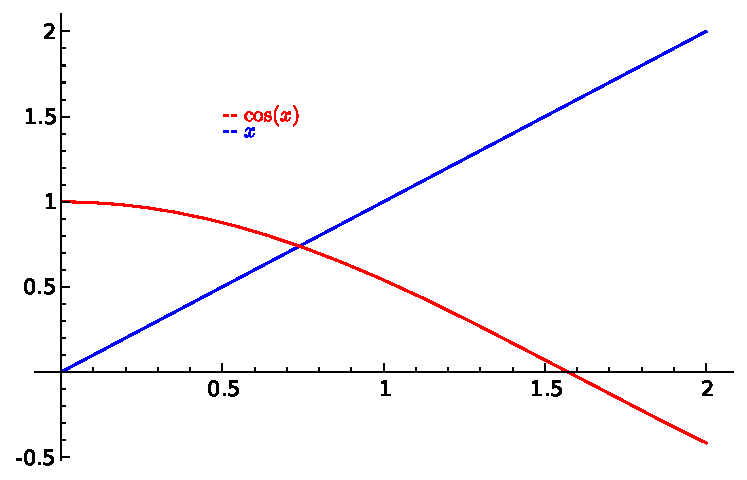
\includegraphics[width=8cm]{figures/iter1.pdf}
\end{center}
\end{frame}

\begin{frame}[fragile]{Fixpunkt-Iteration}
Fixpunkt-Iteration 
\[ x_{k+1}=cos(x_k) \]
bei geeignetem Startwert $x_0 = 0.2$.  \\
\centering{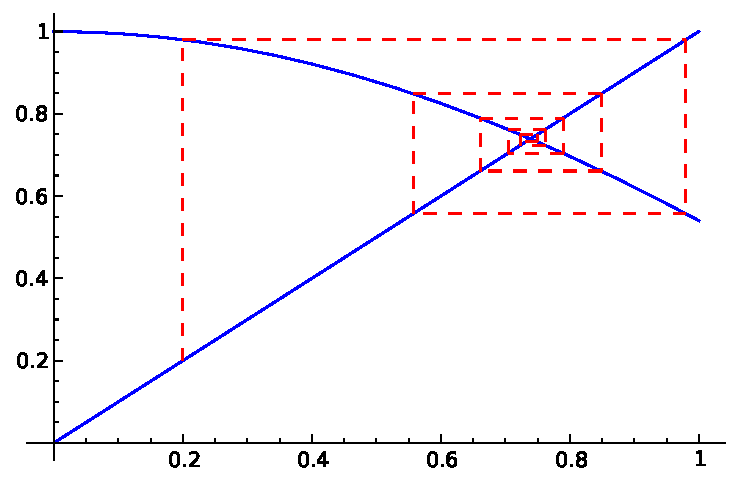
\includegraphics[width=8cm]{figures/fixpunkt.pdf}}\\
\end{frame}

\begin{frame}[fragile]{Implementierung}
\begin{small}
\begin{sage}
>> def fixpunkt(f,In,x0,n):
>>     y = [x0]
>>     p = plot(f,(In[0],In[1]))
>>     p += plot(x,(In[0],In[1]))
>>     for i in [0..n-1]:
>>         y.append(float(f(y[i])))
>>         p += line( [ (y[i],y[i]), (y[i],y[i+1]) ],linestyle='--', color='red')
>>         p += line( [ (y[i],y[i+1]), (y[i+1],y[i+1]) ],linestyle='--', color='red')
>>     p.show()
>>     return(y)
\end{sage}
\end{small}
\end{frame}

\begin{frame}[fragile]{Aufruf}
\begin{sage}
fixpunkt(lambda x: cos(x),[0,1],0.2,10)
\end{sage}
\begin{sage}
[0.200000000000000, 0.98006657784124163, 0.55696725280964243, 0.84886216565827077, 0.66083755111661502, 0.78947843776686832, 0.70421571334199318, 0.76211956176066087, 0.72337417210557109, 0.74957657633149311, 0.73197742525819132]
\end{sage}
\end{frame}










\end{document}
